\documentclass[xcolor=pdftex,dvipsnames,table,aspectratio=169]{beamer}
%\documentclass[xcolor=pdftex,dvipsnames,table,handout,aspectratio=169]{beamer}

%\setbeameroption{show notes}

\usepackage{bm,graphicx,multirow,amsmath,tikz} %fancybox,
\usepackage{color}%,textpos}
\usepackage[round]{natbib}
\usepackage[normalem]{ulem}
\usepackage{hyperref}
\usepackage{lastpage}
\usepackage{array}
\usepackage{color}
\usepackage{framed}
\usepackage{hyperref}

% Define Western colours
\definecolor{western}{rgb}{.306,.152,.524}
\definecolor{westerngray}{rgb}{.512,.508,.524}

%% Define BEAMER colours
\setbeamercolor{frametitle}{bg=western,fg=white}
\setbeamercolor{framesubtitle}{bg=western,fg=black}
\setbeamercolor{title}{fg=white,bg=western}
\setbeamercolor{author}{fg=white,bg=western}
\setbeamercolor{institute}{fg=white,bg=western}
\setbeamercolor{date}{fg=white,bg=western}

%% Set BEAMER fonts
\setbeamerfont{title}{shape=\bf}
\setbeamerfont{frametitle}{shape=\sc,size=\Large}
\setbeamerfont{framesubtitle}{shape=\sc,size=\Large}
\setbeamerfont{footline}{shape=\sc}

%% Define BEAMER toc
\setbeamercolor{section in toc}{fg=western}
\setbeamercolor{subsection in toc}{fg=westerngray}
\setbeamertemplate{sections/subsections in toc}[ball]

%% Define BEAMER background
\setbeamercolor{background canvas}{bg=white}

%% Define BEAMER footer
\setbeamertemplate{navigation symbols}{}
\setbeamercolor{footline}{fg=white,bg=western}
\setbeamertemplate{footline}{%
  \begin{beamercolorbox}[wd=\paperwidth]{footline}
    \vskip5pt

    \raisebox{.05in}{
      \scriptsize{\bf \insertshorttitle}
    }
    \hfill
    \raisebox{.05in}{
      \scriptsize{\bf \insertframenumber/\inserttotalframenumber} 
    }
    \hspace{5pt}

    \vskip5pt
  \end{beamercolorbox}
}

%% Define BLOCK environment
\setbeamercolor{block title}{fg=western}
\setbeamerfont{block title}{series=\bfseries}

%% Define ENUMERATE and ITEMIZE environements
\setbeamertemplate{itemize item}[ball]
\setbeamertemplate{enumerate item}[ball]
\setbeamercolor{item projected}{bg=western}

%% Define BEAMER toc
\setbeamercolor{sections/subsections in toc}{fg=blue!75}
\setbeamertemplate{sections/subsections in toc}[ball]

% %% Define SECTION openings
% \AtBeginSection[]{
%   \begin{frame}{\insertshorttitle}
%     \tableofcontents[currentsection,subsectionstyle=hide/hide/hide]
    
%   \end{frame}
% }

%% Define BEAMER frametitle
\addtobeamertemplate{frametitle}{
   \let\insertframetitle\insertsectionhead}{}
\addtobeamertemplate{frametitle}{
   \let\insertframesubtitle\insertsubsectionhead}{}


\makeatletter
  \CheckCommand*\beamer@checkframetitle{\@ifnextchar\bgroup\beamer@inlineframetitle{}}
  \renewcommand*\beamer@checkframetitle{\global\let\beamer@frametitle\relax\@ifnextchar\bgroup\beamer@inlineframetitle{}}
\makeatother

% Define counters for example and exercise
\newcounter{example}
\newcounter{exercise}

% Define example and exercise commands
\renewcommand{\example}
{\stepcounter{example}Example \lecturenum.\arabic{example}}
\newcommand{\examplectd}
{Example \lecturenum.\arabic{example}\ ctd}
\newcommand{\exercise}
{\stepcounter{exercise}Exercise \lecturenum.\arabic{exercise}}
\newcommand{\exercisectd}
{Exercise \lecturenum.\arabic{exercise}\ ctd}

\newcommand{\lecturenum}{19}

\title[SS2857]{Probability and Statistics I}
\subtitle{\lecturenum.~A Primer on Double Integration}

\date{}

%% Add logo
%% \titlegraphic{\includegraphics[height=2cm]{../uwo_logo_reversed}}

%% Initialize R


\begin{document}

{
\setbeamertemplate{footline}{}
\setbeamercolor{background canvas}{bg=western}

\begin{frame}
  \addtocounter{framenumber}{-1}

  \maketitle
\end{frame}
}


\section{Double Integration}

\begin{frame}

  \begin{block}{Method\footnote{This approach is not completely general but will work for all problems in this course. The method assumes that $y$ is the inner variable of integration and $x$ is the outer variable of integration. The roles would switch if you switch the order of integrations: $\int \int_A f(x,y) ~dx ~dy$.}}
    Suppose that you wish to integrate the function $f(x,y)$ over some domain in $A \subset \mathbb R^2$:
    $$
    \int \int_A f(x,y) ~dy ~dx.
    $$
    \begin{scriptsize}
    \begin{enumerate}[1)]
    \item Sketch the area of integration.
    \item Identify the limits of $y$ as functions of $x$: $l_y(x)$ and $u_y(x)$.
    \item Identify the overall limits of $y$: $l_x$ and $u_x$.
    \item Integrate $f(x,y)$ with respect to $y$ treating $x$ as fixed.
    \item Integrate $g(x)$ with respect to $x$. 
    \end{enumerate}
    \end{scriptsize}
    
  \end{block}
\end{frame}




\begin{frame}
  \begin{block}{\example}
    Integrate $f(x,y)=xy$ over the domain $0<x<1$, $0<y<1$.
    
    \begin{center}
    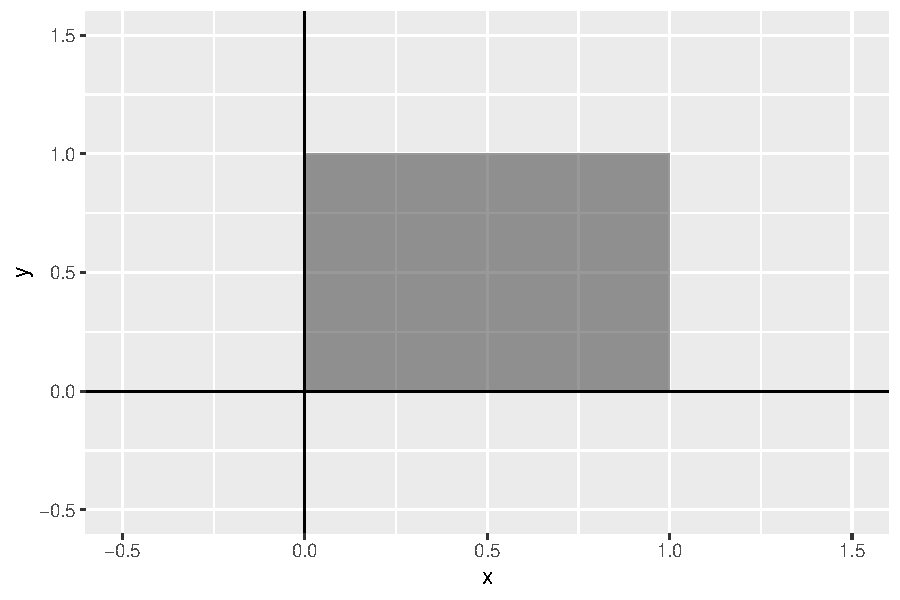
\includegraphics[height = .5\textheight]{figure/example1-1}
    \end{center}
  \end{block}
\end{frame}




\begin{frame}
  \begin{block}{\example}
    Integrate $f(x,y)=xy$ over the domain $x<y<1$, $0<x<1$.
    
    \begin{center}
    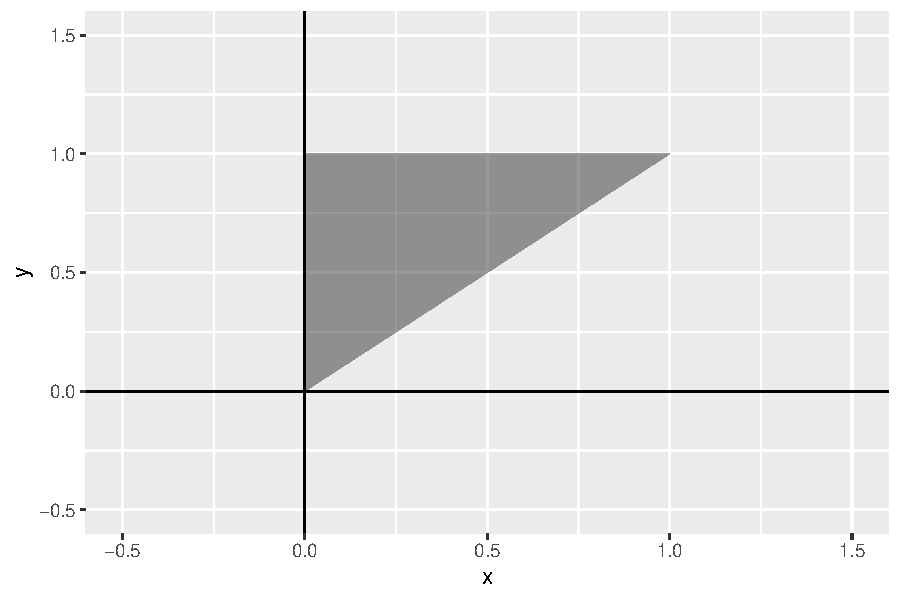
\includegraphics[height = .5\textheight]{figure/example2-1}
    \end{center}
  \end{block}
\end{frame}

 


\begin{frame}
  \begin{block}{\example}
    Integrate $f(x,y)=xy$ over the domain $0 < x < 1$, $0 < x + y < 1$.
  \end{block}
 
 \pause
 
 \begin{center}
    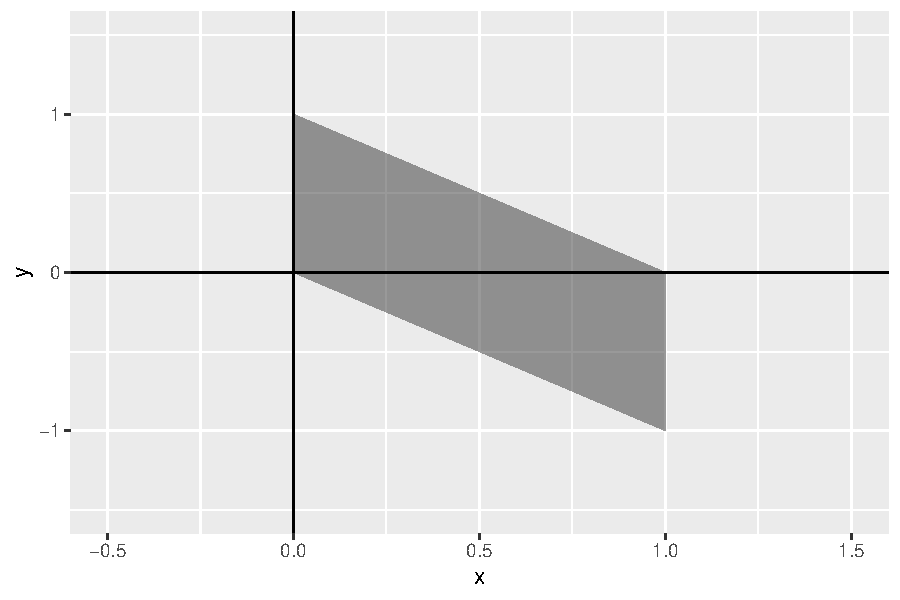
\includegraphics[height = .5\textheight]{figure/example3-1}
    \end{center}
\end{frame}

\begin{frame}

  \begin{block}{Proposition\footnote{Keep in mind that this only works if the domain of $y$ and $x$ do not depend on each other.}}
    Suppose that $f(x,y)=g(x)h(y)$ and the domain of $y$ is independent of $x$ so that $l_y < y < u_y$ regardless of the value of $x$. Then 
\[
  \int_{l_x}^{u_x} \int_{l_y}^{u_y} f(x,y) ~dy ~dx= \int_{l_x}^{u_x} g(x) ~dx \int_{l_y}^{u_y} h(y) ~dy.
\]

  \end{block}
\end{frame}

\begin{frame}
  \begin{block}{\example}
    Integrate $f(x,y)=(1-x^2)(1-y^2)$ over the domain $0<x<1$, $0<y<1$.
  \end{block}
\end{frame}

\begin{frame}<handout:0>
  \begin{center}
    \Huge{\textbf{Questions?}}
  \end{center}
\end{frame}

\begin{frame}

\begin{block}{\exercise}

\begin{enumerate}
\item Integrate $f(x,y)=e^{x+y}-1.
$ over the region $0 < x < 1$, $0<y<1$.
\item Integrate $f(x,y)=e^{x+y}-1.
$ over the region$y < x < 1$, $0 < y < 1$
\item Integrate $f(x,y)=xy$ over the region $x^2 + y^2 < 1$.
\end{enumerate}

\end{block}
\end{frame}

\end{document}
